\documentclass[11pt]{article}

% ---------- Packages (per course conventions) ----------
\usepackage[margin=1in]{geometry}
\usepackage{graphicx}
\usepackage{float}
\usepackage{booktabs}
\usepackage{siunitx}
\usepackage{amsmath}
\usepackage{amssymb}
\usepackage{tikz}
\usetikzlibrary{arrows.meta,calc,patterns,decorations.pathreplacing}
\usepackage{tcolorbox}
\usepackage{enumitem}
\usepackage{xcolor}
\usepackage{hyperref}
\hypersetup{colorlinks=true, linkcolor=black, urlcolor=blue}

\setlength{\parindent}{0pt}
\setlength{\parskip}{0.6\baselineskip}

\newcommand{\assignmentNumber}{7}
\newcommand{\assignedDate}{2 Nov 2026}
\newcommand{\dueDate}{10 Nov 2026 (11:59pm on Moodle)}

% ---------- Boxed-answer helper ----------
\newtcolorbox{finalanswer}{
    colback=white, colframe=black, boxrule=1pt,
    title=Answer, fonttitle=\bfseries, coltitle=black,
    colbacktitle=white
}

% ---------- Units and drawing styles ----------
\newcommand{\un}[1]{\,\text{#1}}
\tikzset{
  force/.style={-{Stealth[length=2.6mm]},thick,red!75!black},
  intl/.style={-{Stealth[length=2.6mm]},thick,blue!70!black},
  load/.style={-{Stealth[length=1.6mm]},semithick},
  moment/.style={-{Stealth[length=2.2mm] Stealth[length=2.2mm]},thick,blue!70!black},
  beam/.style={draw=black,fill=gray!20},
  dimn/.style={{Latex[length=1.6mm]}-{Latex[length=1.6mm]},thin},
  axis/.style={-{Stealth[length=2mm]},thin},
  zero/.style={densely dotted,gray}
}
% small coordinate-axes glyph: \axesglyph{(x,y)}
\newcommand{\axesglyph}[1]{%
  \draw[axis] #1 -- ++(0.7,0) node[right]{\small $x$};
  \draw[axis] #1 -- ++(0,0.7) node[above]{\small $y$};
}

\begin{document}

% =========================================================
% COVERSHEET
% =========================================================
\begin{titlepage}
    \centering
    \vspace*{2cm}
    {\LARGE \bfseries ENGR 225: Mechanics 1} \\[0.3cm]
    {\Large Homework Coversheet} \\[0.3cm]
    {\large Assoc.\ Prof.\ Clayton Byers} \\[2cm]

    \begin{flushleft}
        \Large
        \textbf{NAME:} \underline{\makebox[10cm][l]{\ Sean Balbale}} \\[1cm]
        \textbf{DATE:} \underline{\hspace{10cm}} \\[1cm]
        \textbf{ASSIGNMENT:} \underline{\makebox[9cm][l]{\ Homework 7}} \\[2cm]
    \end{flushleft}

    \large
    \textbf{Level of involvement of AI, LLMs, or related tools in the completion of this assignment:}

    \vspace{1cm}

    \begin{flushleft}
        \Large
        $\square$ \quad None \\[0.7cm]
        $\square$ \quad Minor \\[0.7cm]
        $\square$ \quad Major \\[0.7cm]
        $\square$ \quad Extensive \\[1.5cm]
    \end{flushleft}

    \normalsize
    \textit{Mark the box that applies (e.g., replace $\square$ with $\blacksquare$, or type an X beside it, before compiling/printing). Your disclosure does not affect your grade -- it keeps you accountable for the work you are doing.}

\end{titlepage}

% =========================================================
% HOMEWORK HEADER
% =========================================================
\section*{ENGR 225 -- Homework \assignmentNumber}
\textbf{Assigned:} \assignedDate \hfill \textbf{Due:} \dueDate


Sign convention: $+x$ right, $+y$ up, CCW moments positive. Internal $N$, $V$, $M$ are drawn in their positive sense, so a negative result means the load acts opposite to the direction drawn.

% =========================================================
% PROBLEM 1
% =========================================================
\clearpage
\section*{Problem 1}

\textbf{Given / Find:} Beam $AE$ with a roller at $A$ and a pin at $B$. Measured from $A$: a 500 lb load at 6 ft, point $C$ at 10 ft, $B$ at 14 ft (with a 200 lb load applied at $B$), point $D$ at 20 ft, and a 300 lb load at end $E$ (22 ft). Find the internal shear $V$ and moment $M$ at $C$ and at $D$.

\textbf{Sketch:}

\begin{center}
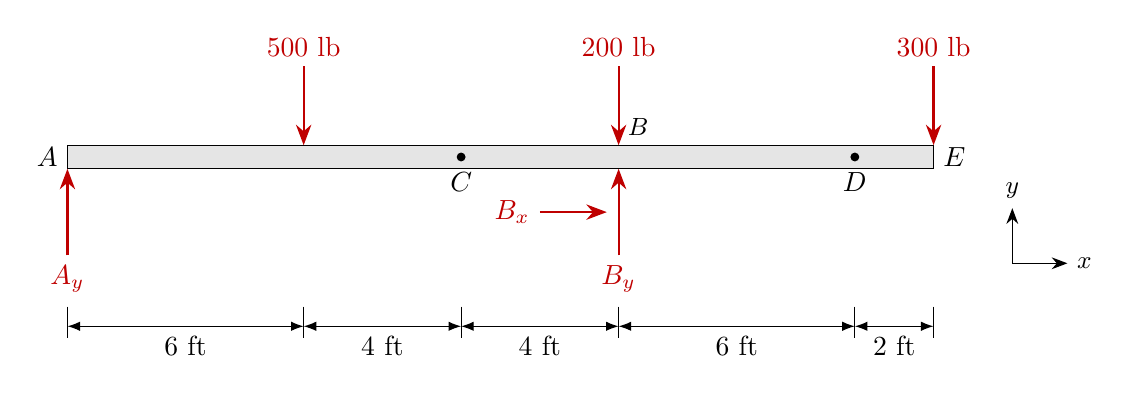
\begin{tikzpicture}[x=1cm,y=1cm]
  % scale: 0.5 cm per ft
  \draw[beam] (0,0) rectangle (11,0.3);
  \node[left] at (0,0.15) {$A$};
  \node[right] at (11,0.15) {$E$};
  % reactions
  \draw[force] (0,-1.1) -- (0,0) node[pos=0,below]{$A_y$};
  \draw[force] (7,-1.1) -- (7,0) node[pos=0,below]{$B_y$};
  \draw[force] (6.0,-0.55) -- (6.85,-0.55) node[pos=0,left]{$B_x$};
  % loads
  \draw[force] (3,1.3) -- (3,0.3) node[pos=0,above]{500 lb};
  \draw[force] (7,1.3) -- (7,0.3) node[pos=0,above]{200 lb};
  \draw[force] (11,1.3) -- (11,0.3) node[pos=0,above]{300 lb};
  \node[above] at (7.25,0.3) {\small $B$};
  % points C, D
  \fill (5,0.15) circle (1.6pt) node[below=2pt]{$C$};
  \fill (10,0.15) circle (1.6pt) node[below=2pt]{$D$};
  % dimensions
  \foreach \p in {0,3,5,7,10,11} \draw[thin] (\p,-1.75) -- (\p,-2.15);
  \draw[dimn] (0,-2) -- (3,-2) node[midway,below]{6 ft};
  \draw[dimn] (3,-2) -- (5,-2) node[midway,below]{4 ft};
  \draw[dimn] (5,-2) -- (7,-2) node[midway,below]{4 ft};
  \draw[dimn] (7,-2) -- (10,-2) node[midway,below]{6 ft};
  \draw[dimn] (10,-2) -- (11,-2) node[midway,below]{2 ft};
  \axesglyph{(12,-1.2)}
\end{tikzpicture}

\vspace{0.4cm}
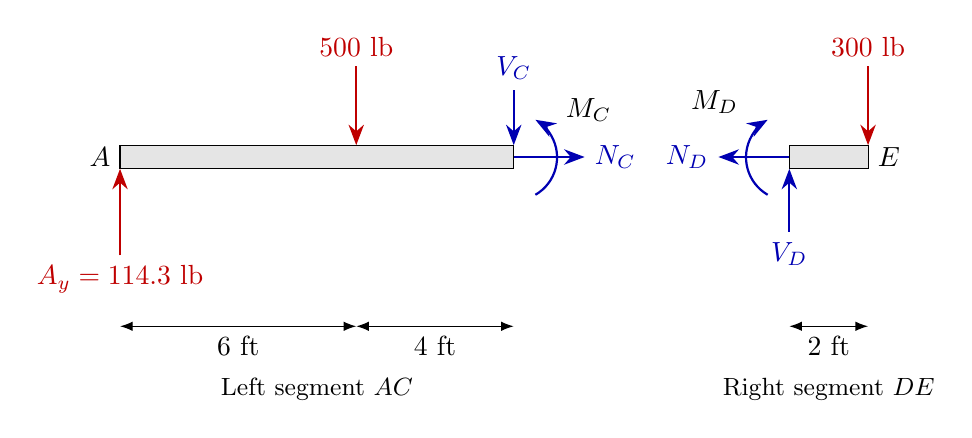
\begin{tikzpicture}[x=1cm,y=1cm]
  % left segment AC
  \draw[beam] (0,0) rectangle (5,0.3);
  \node[left] at (0,0.15) {$A$};
  \draw[force] (0,-1.1) -- (0,0) node[pos=0,below]{$A_y = 114.3$ lb};
  \draw[force] (3,1.3) -- (3,0.3) node[pos=0,above]{500 lb};
  \draw[intl] (5,0.15) -- (5.9,0.15) node[right]{$N_C$};
  \draw[intl] (5,1.0) -- (5,0.3) node[pos=0,above]{$V_C$};
  \draw[intl] (5.275,-0.33) arc (-60:60:0.55);
  \node at (5.95,0.75) {$M_C$};
  \draw[dimn] (0,-2.0) -- (3,-2.0) node[midway,below]{6 ft};
  \draw[dimn] (3,-2.0) -- (5,-2.0) node[midway,below]{4 ft};
  \node at (2.5,-2.8) {\small Left segment $AC$};
  % right segment DE
  \begin{scope}[xshift=8.5cm]
  \draw[beam] (0,0) rectangle (1,0.3);
  \node[right] at (1,0.15) {$E$};
  \draw[force] (1,1.3) -- (1,0.3) node[pos=0,above]{300 lb};
  \draw[intl] (0,0.15) -- (-0.9,0.15) node[left]{$N_D$};
  \draw[intl] (0,-0.8) -- (0,0) node[pos=0,below]{$V_D$};
  \draw[intl] (-0.275,-0.33) arc (240:120:0.55);
  \node at (-0.95,0.85) {$M_D$};
  \draw[dimn] (0,-2.0) -- (1,-2.0) node[midway,below]{2 ft};
  \node at (0.5,-2.8) {\small Right segment $DE$};
  \end{scope}
\end{tikzpicture}
\end{center}

\textbf{Solution:}

\textit{Reactions} ($B_x = 0$):
\begin{align*}
\textstyle\sum M_B &= -A_y(14\un{ft}) + (500\un{lb})(8\un{ft}) - (300\un{lb})(8\un{ft}) = 0\\
A_y &= \frac{4000 - 2400}{14}\un{lb} = 114.3\un{lb}\\[4pt]
\textstyle\sum F_y &= A_y + B_y - 500\un{lb} - 200\un{lb} - 300\un{lb} = 0\\
B_y &= 1000\un{lb} - 114.3\un{lb} = 885.7\un{lb}
\end{align*}

\textit{Section $C$, left segment $AC$:}
\begin{align*}
\textstyle\sum F_y &= 114.3\un{lb} - 500\un{lb} - V_C = 0 \;\Rightarrow\; V_C = -385.7\un{lb}\\
\textstyle\sum M_C &= M_C - (114.3\un{lb})(10\un{ft}) + (500\un{lb})(4\un{ft}) = 0 \;\Rightarrow\; M_C = 1143 - 2000 = -857.1\un{lb\,ft}
\end{align*}

\textit{Section $D$, right segment $DE$:}
\begin{align*}
\textstyle\sum F_y &= V_D - 300\un{lb} = 0 \;\Rightarrow\; V_D = 300\un{lb}\\
\textstyle\sum M_D &= -M_D - (300\un{lb})(2\un{ft}) = 0 \;\Rightarrow\; M_D = -600\un{lb\,ft}
\end{align*}

\begin{finalanswer}
$V_C = -386\un{lb}$, \quad $M_C = -857\un{lb\,ft}$, \qquad $V_D = 300\un{lb}$, \quad $M_D = -600\un{lb\,ft}$
\end{finalanswer}

% =========================================================
% PROBLEM 2
% =========================================================
\clearpage
\section*{Problem 2}

\textbf{Given / Find:} Compound beam: roller at $A$, internal hinge (pin) at $B$, fixed support at $C$. A 6 kip$\cdot$ft counterclockwise couple acts at $A$, a 5 kip load acts 6 ft from $A$ (just right of $D$), $B$ is 12 ft from $A$, and a uniform 1.5 kip/ft load covers $BC$ (8 ft) with $E$ at its midpoint. Find $N$, $V$, and $M$ at sections through $D$ and $E$.

\textbf{Sketch:}

\begin{center}
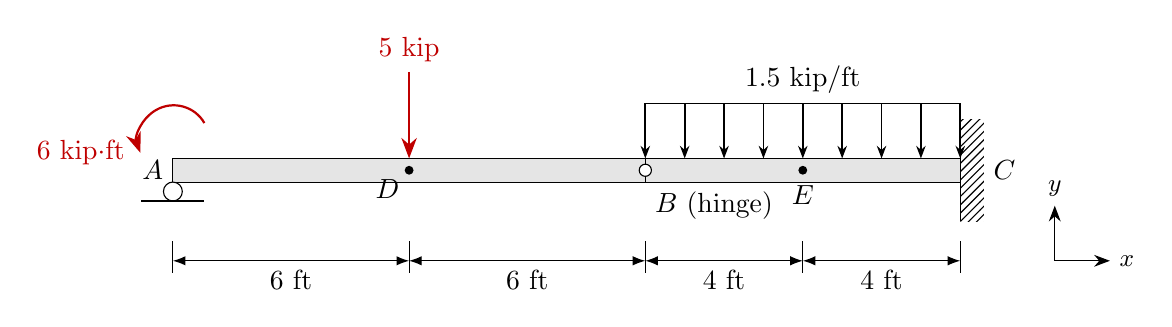
\begin{tikzpicture}[x=1cm,y=1cm]
  % whole beam, 0.5 cm/ft
  \draw[beam] (0,0) rectangle (6,0.3);
  \draw[beam] (6,0) rectangle (10,0.3);
  \fill[pattern=north east lines] (10,-0.5) rectangle (10.3,0.8);
  \draw (10,-0.5) -- (10,0.8);
  \draw[fill=white] (6,0.15) circle (2.2pt);
  \node[below right] at (6,0) {$B$ (hinge)};
  \node[left] at (0,0.15) {$A$};
  \node[right] at (10.3,0.15) {$C$};
  \draw[fill=white] (0,-0.12) circle (0.12);
  \draw (-0.4,-0.24) -- (0.4,-0.24);
  \draw[force] (3,1.4) -- (3,0.3) node[pos=0,above]{5 kip};
  \draw[force] (0.4,0.75) arc (30:200:0.45) node[left=2pt]{6 kip$\cdot$ft};
  \foreach \x in {6,6.5,...,10} \draw[load] (\x,1.0) -- (\x,0.3);
  \draw (6,1.0) -- (10,1.0) node[above,pos=0.5]{1.5 kip/ft};
  \fill (3,0.15) circle (1.6pt) node[below left=0pt]{$D$};
  \fill (8,0.15) circle (1.6pt) node[below=2pt]{$E$};
  \foreach \p in {0,3,6,8,10} \draw[thin] (\p,-0.75) -- (\p,-1.15);
  \draw[dimn] (0,-1) -- (3,-1) node[midway,below]{6 ft};
  \draw[dimn] (3,-1) -- (6,-1) node[midway,below]{6 ft};
  \draw[dimn] (6,-1) -- (8,-1) node[midway,below]{4 ft};
  \draw[dimn] (8,-1) -- (10,-1) node[midway,below]{4 ft};
  \axesglyph{(11.2,-1)}
\end{tikzpicture}

\vspace{0.3cm}
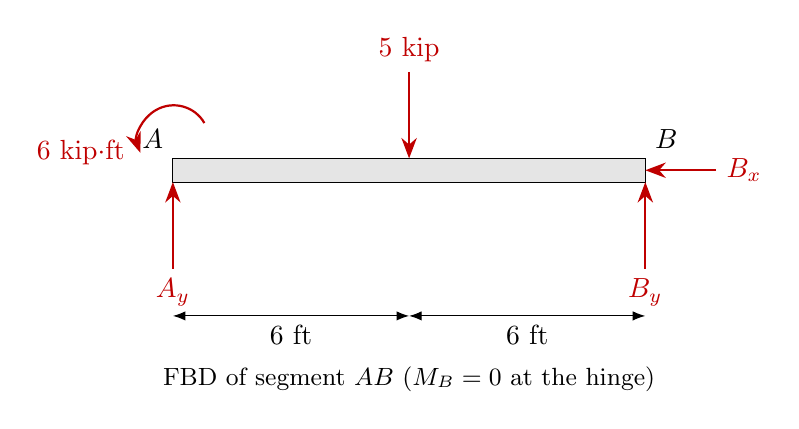
\begin{tikzpicture}[x=1cm,y=1cm]
  % FBD of segment AB
  \draw[beam] (0,0) rectangle (6,0.3);
  \node[above left] at (0,0.3) {$A$}; \node[above right] at (6,0.3) {$B$};
  \draw[force] (0,-1.1) -- (0,0) node[pos=0,below]{$A_y$};
  \draw[force] (6,-1.1) -- (6,0) node[pos=0,below]{$B_y$};
  \draw[force] (6.9,0.15) -- (6,0.15) node[pos=0,right]{$B_x$};
  \draw[force] (3,1.4) -- (3,0.3) node[pos=0,above]{5 kip};
  \draw[force] (0.4,0.75) arc (30:200:0.45) node[left=2pt]{6 kip$\cdot$ft};
  \draw[dimn] (0,-1.7) -- (3,-1.7) node[midway,below]{6 ft};
  \draw[dimn] (3,-1.7) -- (6,-1.7) node[midway,below]{6 ft};
  \node at (3,-2.5) {\small FBD of segment $AB$ ($M_B = 0$ at the hinge)};
\end{tikzpicture}

\vspace{0.3cm}
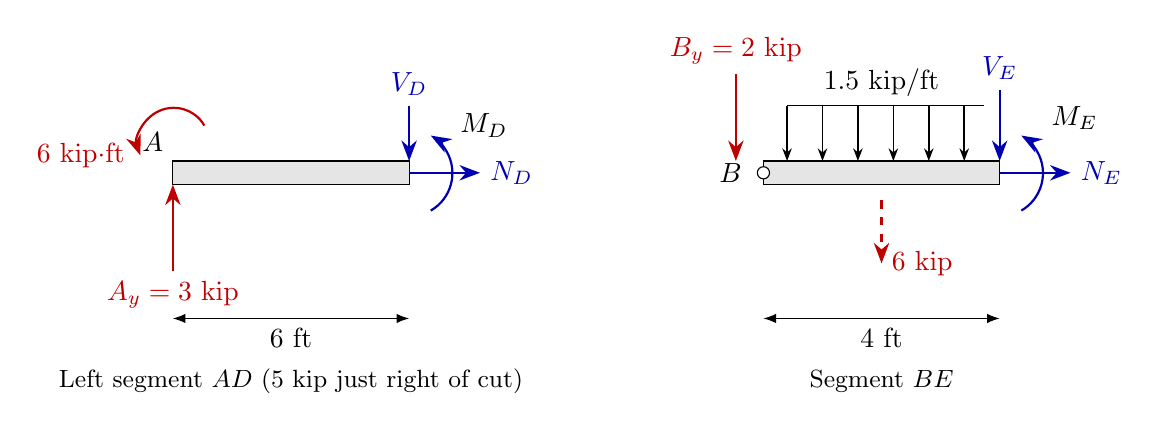
\begin{tikzpicture}[x=1cm,y=1cm]
  % section at D (left segment AD)
  \draw[beam] (0,0) rectangle (3,0.3);
  \node[above left] at (0,0.3) {$A$};
  \draw[force] (0,-1.1) -- (0,0) node[pos=0,below]{$A_y = 3$ kip};
  \draw[force] (0.4,0.75) arc (30:200:0.45) node[left=2pt]{6 kip$\cdot$ft};
  \draw[intl] (3,0.15) -- (3.9,0.15) node[right]{$N_D$};
  \draw[intl] (3,1.0) -- (3,0.3) node[pos=0,above]{$V_D$};
  \draw[intl] (3.275,-0.33) arc (-60:60:0.55);
  \node at (3.95,0.75) {$M_D$};
  \draw[dimn] (0,-1.7) -- (3,-1.7) node[midway,below]{6 ft};
  \node at (1.5,-2.5) {\small Left segment $AD$ (5 kip just right of cut)};
  % section at E (segment BE)
  \begin{scope}[xshift=7.5cm]
  \draw[beam] (0,0) rectangle (3,0.3);
  \draw[fill=white] (0,0.15) circle (2.2pt);
  \node[left] at (-0.15,0.15) {$B$};
  \draw[force] (-0.35,1.4) -- (-0.35,0.3) node[pos=0,above]{$B_y = 2$ kip};
  \foreach \x in {0.3,0.75,...,2.8} \draw[load] (\x,1.0) -- (\x,0.3);
  \draw (0.3,1.0) -- (2.8,1.0);
  \node[above] at (1.5,1.0) {1.5 kip/ft};
  \draw[intl] (3,0.15) -- (3.9,0.15) node[right]{$N_E$};
  \draw[intl] (3,1.2) -- (3,0.3) node[pos=0,above]{$V_E$};
  \draw[intl] (3.275,-0.33) arc (-60:60:0.55);
  \node at (3.95,0.85) {$M_E$};
  \draw[dashed,force] (1.5,-0.2) -- (1.5,-1.0) node[right]{6 kip};
  \draw[dimn] (0,-1.7) -- (3,-1.7) node[midway,below]{4 ft};
  \node at (1.5,-2.5) {\small Segment $BE$};
  \end{scope}
\end{tikzpicture}
\end{center}

\textbf{Solution:}

\textit{Segment $AB$} (hinge: $M_B = 0$):
\begin{align*}
\textstyle\sum M_B &= -A_y(12\un{ft}) + (5\un{kip})(6\un{ft}) + 6\un{kip\,ft} = 0 \;\Rightarrow\; A_y = \frac{36}{12} = 3.00\un{kip}\\
\textstyle\sum F_y &= 3\un{kip} - 5\un{kip} + B_y = 0 \;\Rightarrow\; B_y = 2.00\un{kip}\ \text{(on $AB$)}\\
\textstyle\sum F_x &= B_x = 0
\end{align*}
Hinge force on $BC$: 2.00 kip $\downarrow$.

\textit{Section $D$, left segment $AD$} (5 kip just right of cut):
\begin{align*}
\textstyle\sum F_x &= N_D = 0\\
\textstyle\sum F_y &= 3\un{kip} - V_D = 0 \;\Rightarrow\; V_D = 3.00\un{kip}\\
\textstyle\sum M_D &= M_D - (3\un{kip})(6\un{ft}) + 6\un{kip\,ft} = 0 \;\Rightarrow\; M_D = 12.0\un{kip\,ft}
\end{align*}

\textit{Section $E$, segment $BE$} (distributed resultant $1.5(4) = 6\un{kip}$, 2 ft from $E$):
\begin{align*}
\textstyle\sum F_x &= N_E = 0\\
\textstyle\sum F_y &= -2\un{kip} - 6\un{kip} - V_E = 0 \;\Rightarrow\; V_E = -8.00\un{kip}\\
\textstyle\sum M_E &= M_E + (2\un{kip})(4\un{ft}) + (6\un{kip})(2\un{ft}) = 0 \;\Rightarrow\; M_E = -20.0\un{kip\,ft}
\end{align*}

\begin{finalanswer}
$N_D = 0$, \quad $V_D = 3.00\un{kip}$, \quad $M_D = 12.0\un{kip\,ft}$\\[4pt]
$N_E = 0$, \quad $V_E = -8.00\un{kip}$, \quad $M_E = -20.0\un{kip\,ft}$
\end{finalanswer}

% =========================================================
% PROBLEM 3
% =========================================================
\clearpage
\section*{Problem 3}

\textbf{Given / Find:} Horizontal member $AD$ pinned to the wall at $A$. A vertical post rises 1 m from the member at 2 m from $A$ to point $E$, and a horizontal cable $EB$ ties $E$ back to the wall. At $D$ (4 m from $A$) a 200 N downward load and an 800 N$\cdot$m clockwise couple act. Point $C$ is 1 m from $A$. Find the internal normal force, shear, and moment at $C$.

\textbf{Sketch:}

\begin{center}
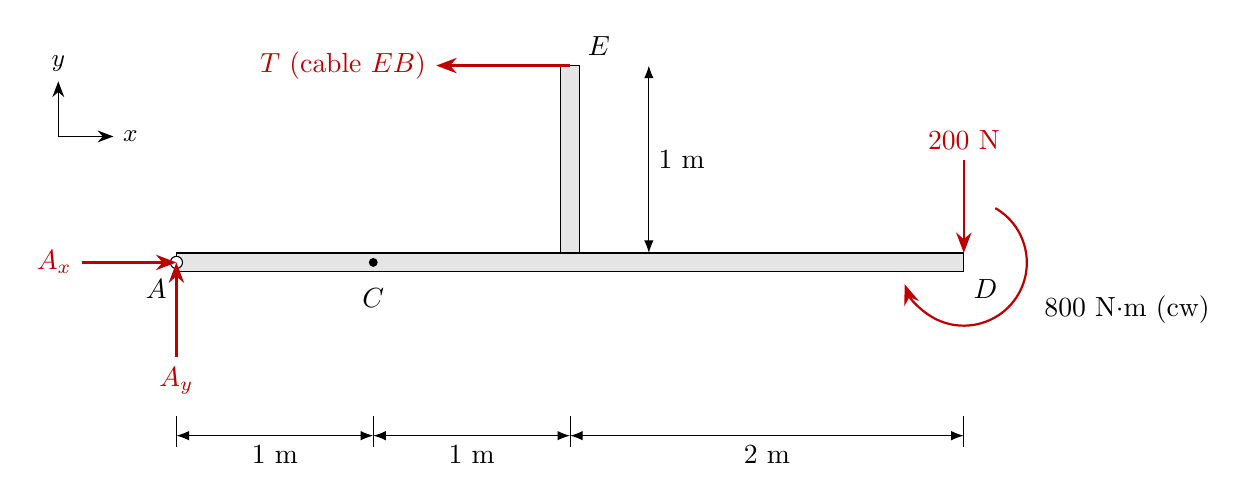
\begin{tikzpicture}[x=1cm,y=1cm]
  % 2.5 cm per m
  \draw[beam] (0,-0.12) rectangle (10,0.12);
  \draw[beam] (4.88,0.12) rectangle (5.12,2.5);
  \draw[fill=white] (0,0) circle (2.2pt); \node[below left] at (0,-0.1) {$A$};
  \fill (2.5,0) circle (1.6pt); \node[below=3pt] at (2.5,-0.1) {$C$};
  \node[above right] at (5.1,2.5) {$E$};
  \node[below right] at (10,-0.1) {$D$};
  % forces
  \draw[force] (-1.2,0) -- (0,0) node[pos=0,left]{$A_x$};
  \draw[force] (0,-1.2) -- (0,0) node[pos=0,below]{$A_y$};
  \draw[force] (5,2.5) -- (3.3,2.5) node[left]{$T$ (cable $EB$)};
  \draw[force] (10,1.3) -- (10,0.12) node[pos=0,above]{200 N};
  \draw[force] (10.4,0.69) arc (60:-160:0.8);
  \node[right] at (10.9,-0.6) {800 N$\cdot$m (cw)};
  % dims
  \foreach \p in {0,2.5,5,10} \draw[thin] (\p,-1.95) -- (\p,-2.35);
  \draw[dimn] (0,-2.2) -- (2.5,-2.2) node[midway,below]{1 m};
  \draw[dimn] (2.5,-2.2) -- (5,-2.2) node[midway,below]{1 m};
  \draw[dimn] (5,-2.2) -- (10,-2.2) node[midway,below]{2 m};
  \draw[dimn] (6,0.12) -- (6,2.5) node[midway,right]{1 m};
  \axesglyph{(-1.5,1.6)}
\end{tikzpicture}

\vspace{0.4cm}
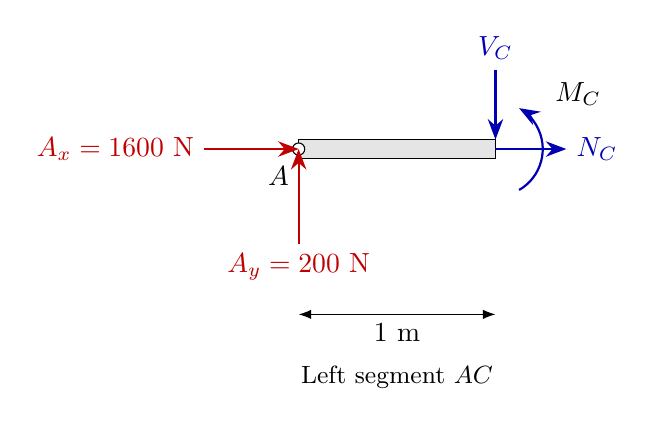
\begin{tikzpicture}[x=1cm,y=1cm]
  \draw[beam] (0,-0.12) rectangle (2.5,0.12);
  \draw[fill=white] (0,0) circle (2.2pt); \node[below left] at (0,-0.1) {$A$};
  \draw[force] (-1.2,0) -- (0,0) node[pos=0,left]{$A_x = 1600$ N};
  \draw[force] (0,-1.2) -- (0,0) node[pos=0,below]{$A_y = 200$ N};
  \draw[intl] (2.5,0) -- (3.4,0) node[right]{$N_C$};
  \draw[intl] (2.5,1.0) -- (2.5,0.12) node[pos=0,above]{$V_C$};
  \draw[intl] (2.8,-0.52) arc (-60:60:0.6);
  \node at (3.55,0.7) {$M_C$};
  \draw[dimn] (0,-2.1) -- (2.5,-2.1) node[midway,below]{1 m};
  \node at (1.25,-2.9) {\small Left segment $AC$};
\end{tikzpicture}
\end{center}

\textbf{Solution:}

\textit{Whole frame} ($T$ horizontal at $E$, 1 m above $AD$):
\begin{align*}
\textstyle\sum M_A &= T(1\un{m}) - (200\un{N})(4\un{m}) - 800\un{N\,m} = 0 \;\Rightarrow\; T = 1600\un{N}\\
\textstyle\sum F_x &= A_x - 1600\un{N} = 0 \;\Rightarrow\; A_x = 1600\un{N}\\
\textstyle\sum F_y &= A_y - 200\un{N} = 0 \;\Rightarrow\; A_y = 200\un{N}
\end{align*}

\textit{Section $C$, left segment $AC$:}
\begin{align*}
\textstyle\sum F_x &= 1600\un{N} + N_C = 0 \;\Rightarrow\; N_C = -1600\un{N}\ \text{(compression)}\\
\textstyle\sum F_y &= 200\un{N} - V_C = 0 \;\Rightarrow\; V_C = 200\un{N}\\
\textstyle\sum M_C &= M_C - (200\un{N})(1\un{m}) = 0 \;\Rightarrow\; M_C = 200\un{N\,m}
\end{align*}

\begin{finalanswer}
$N_C = -1.60\un{kN}$ (compression), \quad $V_C = 200\un{N}$, \quad $M_C = 200\un{N\,m}$
\end{finalanswer}

% =========================================================
% PROBLEM 4
% =========================================================
\clearpage
\section*{Problem 4}

\textbf{Given / Find:} L-shaped pipe fixed at $A$. Segment $A$-to-elbow runs 2 m along $x$, with $B$ at its midpoint (1 m from $A$). From the elbow, a 1.5 m segment runs in the $+y$ direction. $\vec F_2 = (100\hat\imath + 500\hat\jmath)$ N acts at the elbow (labeled $C$ here) and $\vec F_1 = (100\hat\imath - 200\hat\jmath - 300\hat k)$ N acts at the free end (labeled $D$ here). Pipe weight is neglected. Find the $x$, $y$, $z$ components of internal force and moment at a section through $B$.

\textbf{Sketch:}

\begin{center}
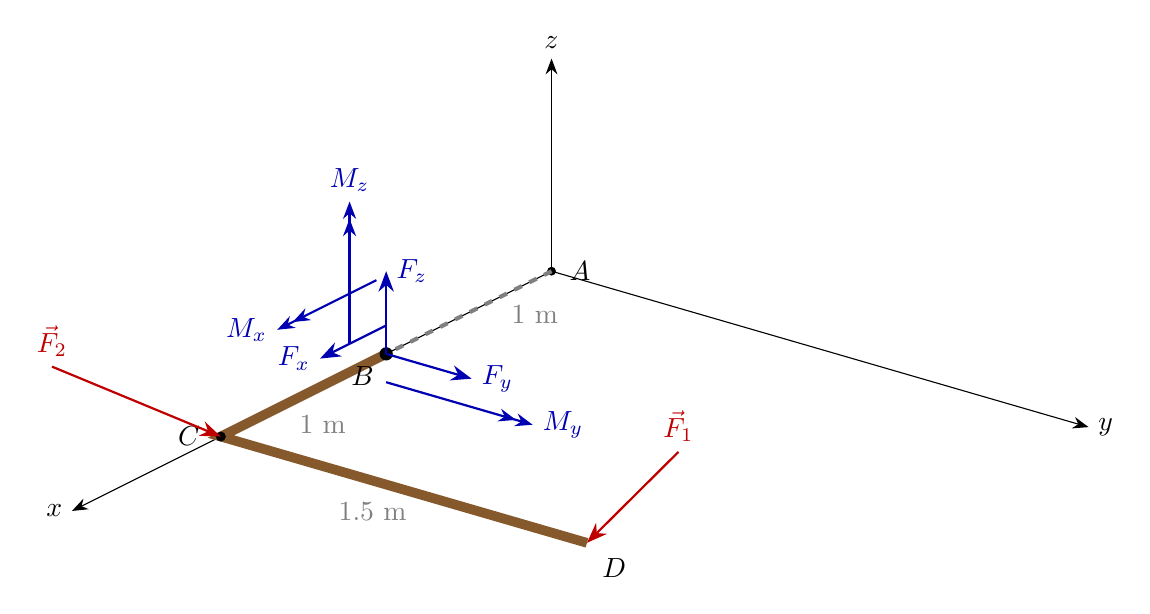
\begin{tikzpicture}[x={(-2.1cm,-1.05cm)},y={(3.1cm,-0.9cm)},z={(0cm,3.0cm)}]
  % axes at A (same view as the problem figure)
  \draw[axis] (0,0,0) -- (2.9,0,0) node[left]{$x$};
  \draw[axis] (0,0,0) -- (0,2.2,0) node[right]{$y$};
  \draw[axis] (0,0,0) -- (0,0,0.9) node[above]{$z$};
  \fill (0,0,0) circle (1.6pt);
  \node[right=3pt] at (0,0,0) {$A$};
  % segment AB removed (support not part of this FBD)
  \draw[dashed,gray,line width=1.5pt] (0,0,0) -- (1,0,0);
  % free body BCD
  \draw[line width=3.5pt,brown!70!black] (1,0,0) -- (2,0,0) -- (2,1.5,0);
  \fill (1,0,0) circle (2.4pt);
  \node[below left=1pt] at (1,0,0) {$B$};
  \fill (2,0,0) circle (1.8pt);
  \node[left=4pt] at (2,0,0) {$C$};
  \node[below right=2pt] at (2,1.5,0) {$D$};
  % dimensions
  \node[gray,below right] at (0.3,0,0) {1 m};
  \node[gray,below right=1pt] at (1.6,0,0) {1 m};
  \node[gray,below left] at (2,0.8,0) {1.5 m};
  % applied loads, direction to scale: F2 ~ (1,5,0), F1 ~ (1,-2,-3)
  \draw[force] ($(2,0,0)-0.16*(1,5,0)$) -- (2,0,0) node[pos=0,above]{$\vec F_2$};
  \draw[force] ($(2,1.5,0)-0.14*(1,-2,-3)$) -- (2,1.5,0) node[pos=0,above]{$\vec F_1$};
  % internal loads at B, each drawn in its + axis direction
  \draw[intl] (1,0,0.12) -- (1.4,0,0.12) node[left]{$F_{x}$};
  \draw[intl] (1,0,0) -- (1,0.35,0) node[right]{$F_{y}$};
  \draw[intl] (1,0,0) -- (1,0,0.35) node[right]{$F_{z}$};
  \draw[moment] (1,-0.04,0.3) -- (1.6,-0.04,0.3) node[left]{$M_{x}$};
  \draw[moment] (1,0,-0.12) -- (1,0.6,-0.12) node[right]{$M_{y}$};
  \draw[moment] (1,-0.15,0) -- (1,-0.15,0.6) node[above]{$M_{z}$};
\end{tikzpicture}

{\small FBD of segment $BCD$ ($C$ = elbow, $D$ = free end). Internal loads at $B$ drawn in the $+x$, $+y$, $+z$ directions (single arrow = force, double arrow = moment); a negative answer means the actual load points the other way.}
\end{center}

\textbf{Solution:}

\textit{Outboard segment $BCD$}, position vectors from $B$:
\[
\vec r_{BC} = (1\hat\imath)\un{m}, \qquad \vec r_{BD} = (1\hat\imath + 1.5\hat\jmath)\un{m}
\]

\textit{Force equilibrium:}
\begin{align*}
\textstyle\sum \vec F &= \vec F_B + \vec F_1 + \vec F_2 = 0\\
\vec F_B &= -\big[(100+100)\hat\imath + (-200+500)\hat\jmath + (-300)\hat k\big]\un{N}\\
&= (-200\hat\imath - 300\hat\jmath + 300\hat k)\un{N}
\end{align*}

\textit{Moment equilibrium about $B$:}
\begin{align*}
\textstyle\sum \vec M_B &= \vec M_B + \vec r_{BD}\times\vec F_1 + \vec r_{BC}\times\vec F_2 = 0\\[4pt]
\vec r_{BD}\times\vec F_1 = \begin{vmatrix}\hat\imath & \hat\jmath & \hat k\\ 1 & 1.5 & 0\\ 100 & -200 & -300\end{vmatrix}
&= \big[(1.5)(-300) - (0)(-200)\big]\hat\imath - \big[(1)(-300) - (0)(100)\big]\hat\jmath\\
&\qquad + \big[(1)(-200) - (1.5)(100)\big]\hat k\\
&= (-450\hat\imath + 300\hat\jmath - 350\hat k)\un{N\,m}\\[4pt]
\vec r_{BC}\times\vec F_2 = \begin{vmatrix}\hat\imath & \hat\jmath & \hat k\\ 1 & 0 & 0\\ 100 & 500 & 0\end{vmatrix}
&= (0)\hat\imath - (0)\hat\jmath + \big[(1)(500) - (0)(100)\big]\hat k\\ &= (500\hat k)\un{N\,m}\\[4pt]
\vec M_B &= -\big[-450\hat\imath + 300\hat\jmath + (-350+500)\hat k\big]\un{N\,m}\\
&= (450\hat\imath - 300\hat\jmath - 150\hat k)\un{N\,m}
\end{align*}


\begin{finalanswer}
$F_x = -200\un{N}$, \quad $F_y = -300\un{N}$, \quad $F_z = 300\un{N}$\\[4pt]
$M_x = 450\un{N\,m}$, \quad $M_y = -300\un{N\,m}$, \quad $M_z = -150\un{N\,m}$
\end{finalanswer}

% =========================================================
% PROBLEM 5
% =========================================================
\clearpage
\section*{Problem 5}

\textbf{Given / Find:} 24 ft cantilever fixed at $A$ ($x=0$) carrying a triangular distributed load that rises from 0 at $A$ to 4 kip/ft at $x = 12$ ft and falls back to 0 at the free end ($x = 24$ ft). Find $V(x)$ and $M(x)$ for both regions and draw the shear and moment diagrams.

\textbf{Sketch:}

\begin{center}
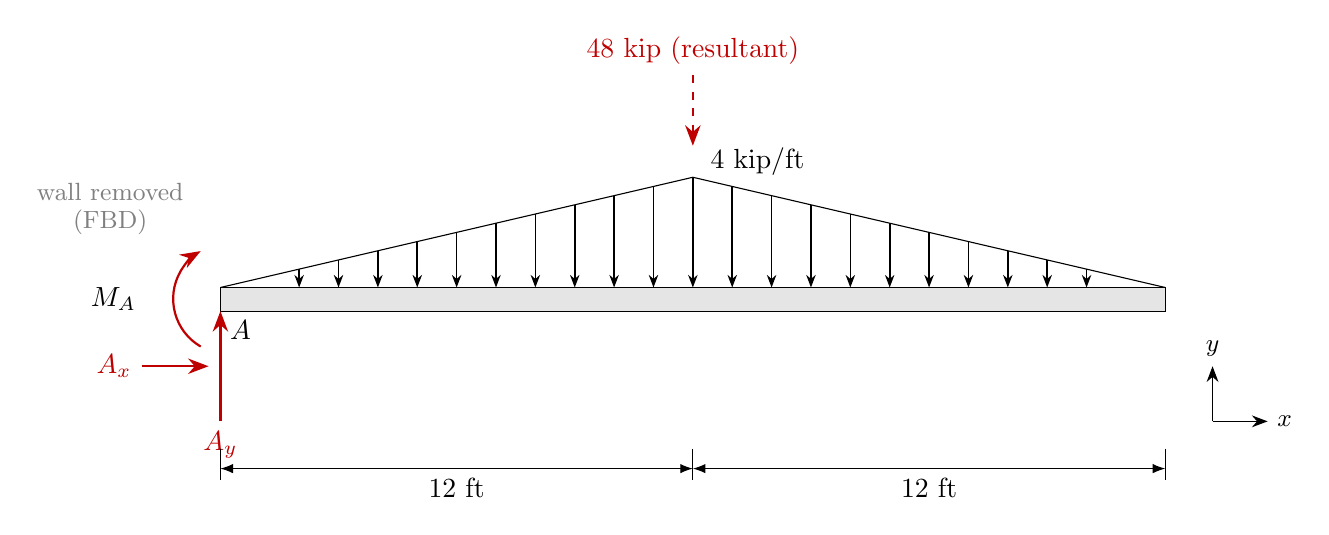
\begin{tikzpicture}[x=1cm,y=1cm]
  % 0.5 cm per ft
  \draw[beam] (0,0) rectangle (12,0.3);
  \node[below right] at (0,0) {$A$};
  \node[gray,align=center] at (-1.4,1.3) {\small wall removed\\[-2pt]\small (FBD)};
  \draw (0,0.3) -- (6,1.7) -- (12,0.3);
  \foreach \x in {1,1.5,...,11} {
    \pgfmathsetmacro{\h}{1.4*(1-abs(\x-6)/6)}
    \draw[load] (\x,0.3+\h) -- (\x,0.3);
  }
  \node[above right] at (6.1,1.6) {4 kip/ft};
  \draw[force,dashed] (6,3.0) -- (6,2.1) node[pos=0,above]{48 kip (resultant)};
  \draw[force] (0,-1.4) -- (0,0) node[pos=0,below]{$A_y$};
  \draw[force] (-0.25,-0.45) arc (240:120:0.7);
  \node[left] at (-0.95,0.15) {$M_A$};
  \draw[force] (-1.0,-0.7) -- (-0.15,-0.7) node[pos=0,left]{$A_x$};
  \foreach \p in {0,6,12} \draw[thin] (\p,-1.75) -- (\p,-2.15);
  \draw[dimn] (0,-2) -- (6,-2) node[midway,below]{12 ft};
  \draw[dimn] (6,-2) -- (12,-2) node[midway,below]{12 ft};
  \axesglyph{(12.6,-1.4)}
\end{tikzpicture}
\end{center}

\textbf{Solution:}

\textit{Reactions:} $F_R = \tfrac12(24)(4) = 48\un{kip}$ at $x = 12$ ft; $A_x = 0$.
\begin{align*}
\textstyle\sum F_y &= A_y - 48\un{kip} = 0 \;\Rightarrow\; A_y = 48.0\un{kip}\\
\textstyle\sum M_A &= M_A - (48\un{kip})(12\un{ft}) = 0 \;\Rightarrow\; M_A = 576\un{kip\,ft}
\end{align*}
So $M(0) = -576\un{kip\,ft}$.

$w(x) = \tfrac{x}{3}$ ($0 \le x \le 12$), \quad $w(x) = \tfrac{24-x}{3}$ ($12 \le x \le 24$) kip/ft.

\textit{Region 1, $0 \le x \le 12$ (left segment):} load $\tfrac{x^2}{6}$ kip at $\tfrac{x}{3}$ from cut.
\begin{align*}
\textstyle\sum F_y &= 48 - \frac{x^2}{6} - V = 0 \;\Rightarrow\; V(x) = -\frac{1}{6}x^2 + 48 \quad \text{(kip)}\\
\textstyle\sum M_{\text{cut}} &= M + 576 - 48x + \frac{x^2}{6}\cdot\frac{x}{3} = 0\\ M(x) &= -\frac{1}{18}x^3 + 48x - 576 \quad \text{(kip$\cdot$ft)}
\end{align*}

\textit{Region 2, $12 \le x \le 24$ (right segment):} load $\tfrac{(24-x)^2}{6}$ kip at $\tfrac{24-x}{3}$ from cut.
\begin{align*}
\textstyle\sum F_y &= V - \frac{(24-x)^2}{6} = 0 \;\Rightarrow\; V(x) = \frac{1}{6}x^2 - 8x + 96 \quad \text{(kip)}\\\\
\textstyle\sum M_{\text{cut}} &= -M - \frac{(24-x)^2}{6}\cdot\frac{24-x}{3} = 0 \;\Rightarrow\; M(x) = -\frac{(24-x)^3}{18}\\
M(x) &= \frac{1}{18}x^3 - 4x^2 + 96x - 768 \quad \text{(kip$\cdot$ft)}
\end{align*}

\textit{Critical values:}
\begin{align*}
V(0) &= 48.0\un{kip}, & V(12) &= 24.0\un{kip}, & V(24) &= 0\\
M(0) &= -576\un{kip\,ft}, & M(12) &= -96.0\un{kip\,ft}, & M(24) &= 0
\end{align*}
$dV/dx = -w \le 0$ and $dM/dx = V \ge 0$ on $0 < x < 24$: no interior zero crossings.

\noindent\begin{minipage}{\linewidth}
\textbf{Shear and moment diagrams:}

\begin{center}
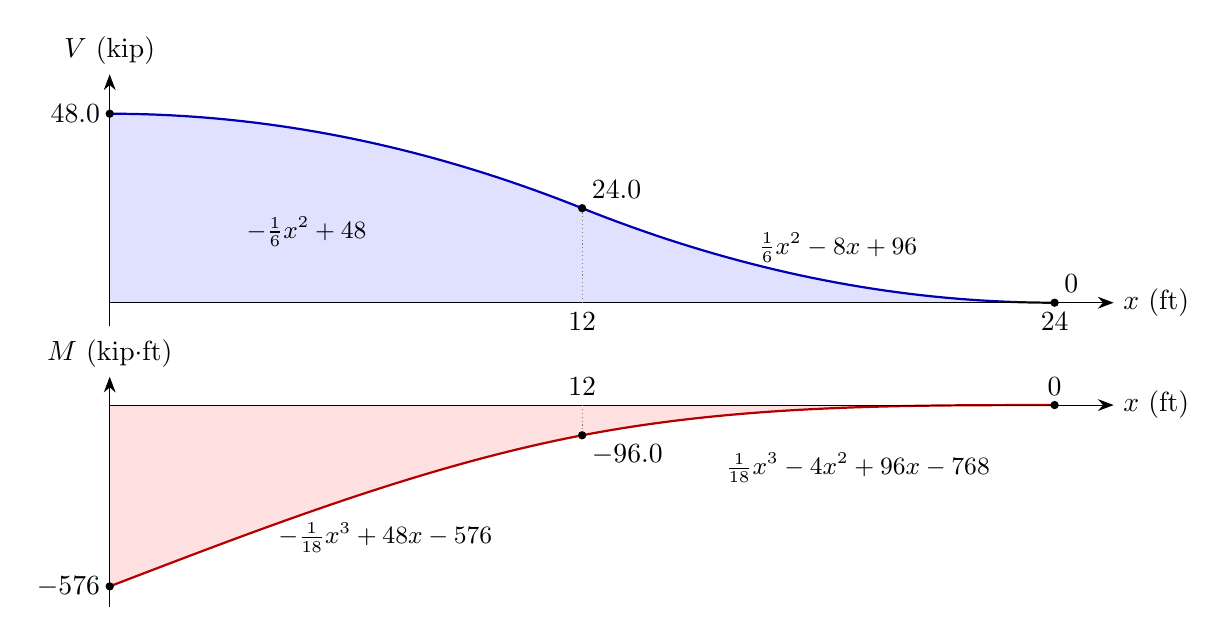
\begin{tikzpicture}[x=1cm,y=1cm]
  % --- V diagram ---
  \begin{scope}[x=0.5cm,y=0.05cm]
    \fill[blue!12] (0,0) -- plot[domain=0:12,samples=40] (\x,{48-\x*\x/6}) -- plot[domain=12:24,samples=40] (\x,{\x*\x/6-8*\x+96}) -- (24,0) -- cycle;
    \draw[thick,blue!70!black] plot[domain=0:12,samples=40] (\x,{48-\x*\x/6});
    \draw[thick,blue!70!black] plot[domain=12:24,samples=40] (\x,{\x*\x/6-8*\x+96});
    \draw[axis] (0,0) -- (25.5,0) node[right]{$x$ (ft)};
    \draw[axis] (0,-6) -- (0,58) node[above]{$V$ (kip)};
    \draw[zero] (12,0) -- (12,24);
    \fill (0,48) circle (1.5pt) node[left]{48.0};
    \fill (12,24) circle (1.5pt) node[above right]{24.0};
    \fill (24,0) circle (1.5pt) node[above right]{0};
    \node[below] at (12,0) {12};
    \node[below] at (24,0) {24};
    \node at (5,18) {\small $-\tfrac16x^2+48$};
    \node at (18.5,14) {\small $\tfrac16x^2-8x+96$};
  \end{scope}
  % --- M diagram ---
  \begin{scope}[yshift=-1.3cm,x=0.5cm,y=0.004cm]
    \fill[red!12] (0,0) -- plot[domain=0:12,samples=40] (\x,{-\x*\x*\x/18+48*\x-576}) -- plot[domain=12:24,samples=40] (\x,{-(24-\x)*(24-\x)*(24-\x)/18}) -- (24,0) -- cycle;
    \draw[thick,red!70!black] plot[domain=0:12,samples=40] (\x,{-\x*\x*\x/18+48*\x-576});
    \draw[thick,red!70!black] plot[domain=12:24,samples=40] (\x,{-(24-\x)*(24-\x)*(24-\x)/18});
    \draw[axis] (0,0) -- (25.5,0) node[right]{$x$ (ft)};
    \draw[axis] (0,-640) -- (0,90) node[above]{$M$ (kip$\cdot$ft)};
    \draw[zero] (12,0) -- (12,-96);
    \fill (0,-576) circle (1.5pt) node[left]{$-576$};
    \fill (12,-96) circle (1.5pt) node[below right]{$-96.0$};
    \fill (24,0) circle (1.5pt) node[above]{0};
    \node[above] at (12,0) {12};
    \node at (7,-420) {\small $-\tfrac1{18}x^3+48x-576$};
    \node at (19,-200) {\small $\tfrac1{18}x^3-4x^2+96x-768$};
  \end{scope}
\end{tikzpicture}
\end{center}
\end{minipage}

\begin{finalanswer}
$0 \le x \le 12$ ft: \quad $V(x) = -\tfrac16 x^2 + 48$ kip, \quad $M(x) = -\tfrac1{18}x^3 + 48x - 576$ kip$\cdot$ft\\[4pt]
$12 \le x \le 24$ ft: \quad $V(x) = \tfrac16 x^2 - 8x + 96$ kip, \quad $M(x) = \tfrac1{18}x^3 - 4x^2 + 96x - 768$ kip$\cdot$ft\\[4pt]
$V_{\max} = 48.0$ kip and $M_{\min} = -576$ kip$\cdot$ft, both at $x = 0$ (wall); $V(12) = 24.0$ kip, $M(12) = -96.0$ kip$\cdot$ft; $V = M = 0$ at $x = 24$ ft.
\end{finalanswer}

% =========================================================
% PROBLEM 6
% =========================================================
\clearpage
\section*{Problem 6}

\textbf{Given / Find:} Beam with a pin at $A$ ($x = 0$), a roller at $B$ ($x = 6$ ft), and an overhang to $C$ ($x = 9$ ft). A triangular load rises from 0 at $A$ to 3 kip/ft at $B$; a uniform 2 kip/ft load covers $BC$. Find $V(x)$ and $M(x)$ and draw the shear and moment diagrams.

\textbf{Sketch:}

\begin{center}
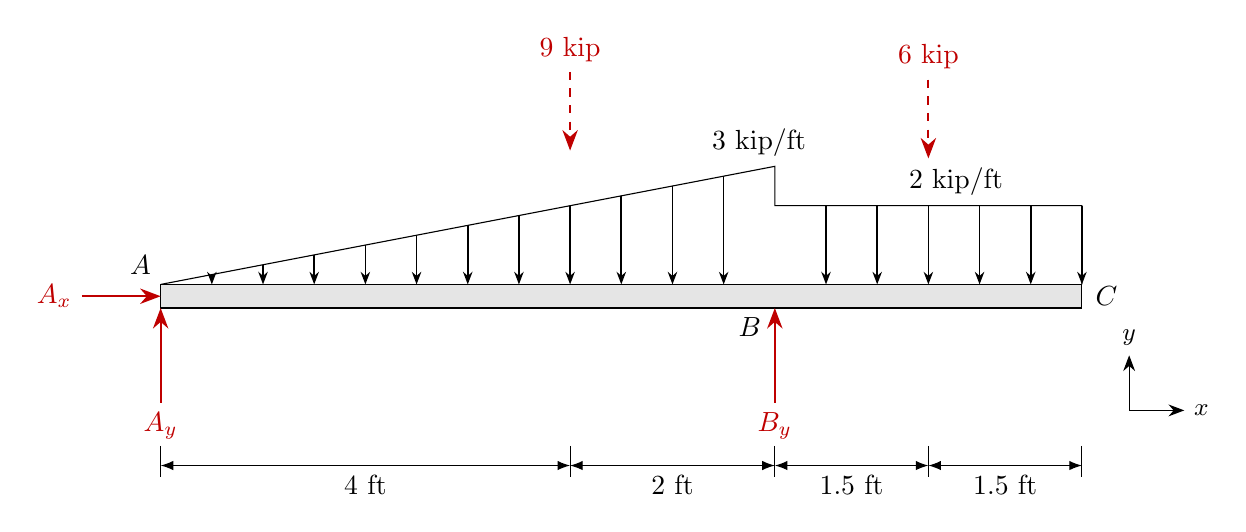
\begin{tikzpicture}[x=1cm,y=1cm]
  % 1.3 cm per ft
  \draw[beam] (0,0) rectangle (11.7,0.3);
  \node[above left] at (0,0.3) {$A$};
  \node[right] at (11.75,0.15) {$C$};
  \draw (0,0.3) -- (7.8,1.8) -- (7.8,1.3) -- (11.7,1.3) -- (11.7,0.3);
  \foreach \x in {0.65,1.3,...,7.8} {
    \pgfmathsetmacro{\h}{1.5*\x/7.8}
    \draw[load] (\x,0.3+\h) -- (\x,0.3);
  }
  \foreach \x in {8.45,9.1,...,11.75} \draw[load] (\x,1.3) -- (\x,0.3);
  \node[above] at (7.6,1.8) {3 kip/ft};
  \node[above] at (10.1,1.3) {2 kip/ft};
  \draw[force,dashed] (5.2,3.0) -- (5.2,2.0) node[pos=0,above]{9 kip};
  \draw[force,dashed] (9.75,2.9) -- (9.75,1.9) node[pos=0,above]{6 kip};
  \draw[force] (0,-1.2) -- (0,0) node[pos=0,below]{$A_y$};
  \draw[force] (-1.0,0.15) -- (0,0.15) node[pos=0,left]{$A_x$};
  \draw[force] (7.8,-1.2) -- (7.8,0) node[pos=0,below]{$B_y$};
  \node[below left] at (7.75,0) {$B$};
  \foreach \p in {0,5.2,7.8,9.75,11.7} \draw[thin] (\p,-1.75) -- (\p,-2.15);
  \draw[dimn] (0,-2) -- (5.2,-2) node[midway,below]{4 ft};
  \draw[dimn] (5.2,-2) -- (7.8,-2) node[midway,below]{2 ft};
  \draw[dimn] (7.8,-2) -- (9.75,-2) node[midway,below]{1.5 ft};
  \draw[dimn] (9.75,-2) -- (11.7,-2) node[midway,below]{1.5 ft};
  \axesglyph{(12.3,-1.3)}
\end{tikzpicture}
\end{center}

\textbf{Solution:}

\textit{Reactions:} triangle $\tfrac12(6)(3) = 9\un{kip}$ at 4 ft; uniform $2(3) = 6\un{kip}$ at 7.5 ft; $A_x = 0$.
\begin{align*}
\textstyle\sum M_A &= B_y(6\un{ft}) - (9\un{kip})(4\un{ft}) - (6\un{kip})(7.5\un{ft}) = 0 \;\Rightarrow\; B_y = \frac{36 + 45}{6} = 13.5\un{kip}\\
\textstyle\sum F_y &= A_y + 13.5 - 9 - 6 = 0 \;\Rightarrow\; A_y = 1.50\un{kip}
\end{align*}

\textit{Region 1, $0 \le x < 6$ (left segment):} $w = \tfrac{x}{2}$, load $\tfrac{x^2}{4}$ kip at $\tfrac{x}{3}$ from cut.
\begin{align*}
\textstyle\sum F_y &= 1.5 - \frac{x^2}{4} - V = 0 \;\Rightarrow\; V(x) = -\frac14 x^2 + 1.5 \quad \text{(kip)}\\
\textstyle\sum M_{\text{cut}} &= M - 1.5x + \frac{x^2}{4}\cdot\frac{x}{3} = 0 \;\Rightarrow\; M(x) = -\frac{1}{12}x^3 + 1.5x \quad \text{(kip$\cdot$ft)}
\end{align*}

\textit{Region 2, $6 < x \le 9$ (right segment):} load $2(9-x)$ kip at $\tfrac{9-x}{2}$ from cut.
\begin{align*}
\textstyle\sum F_y &= V - 2(9-x) = 0 \;\Rightarrow\; V(x) = -2x + 18 \quad \text{(kip)}\\
\textstyle\sum M_{\text{cut}} &= -M - 2(9-x)\cdot\frac{9-x}{2} = 0\\ M(x) &= -(9-x)^2 = -x^2 + 18x - 81 \quad \text{(kip$\cdot$ft)}
\end{align*}

\textit{Critical values:}
\begin{align*}
V = 0:\ -\tfrac14x^2 + 1.5 = 0 &\Rightarrow x = 2.45\un{ft},\quad M_{\max} = -\tfrac1{12}(2.449)^3 + 1.5(2.449) = 2.45\un{kip\,ft}\\
M = 0:\ -\tfrac1{12}x^3 + 1.5x = 0 &\Rightarrow x = \sqrt{18} = 4.24\un{ft}\\
x = 6:\ V(6^-) = -7.50\un{kip},\ V(6^+) &= 6.00\un{kip}\ (\Delta V = B_y),\quad M(6) = -9.00\un{kip\,ft}\\
x = 9:\ V &= 0,\quad M = 0
\end{align*}

\noindent\begin{minipage}{\linewidth}
\textbf{Shear and moment diagrams:}

\begin{center}
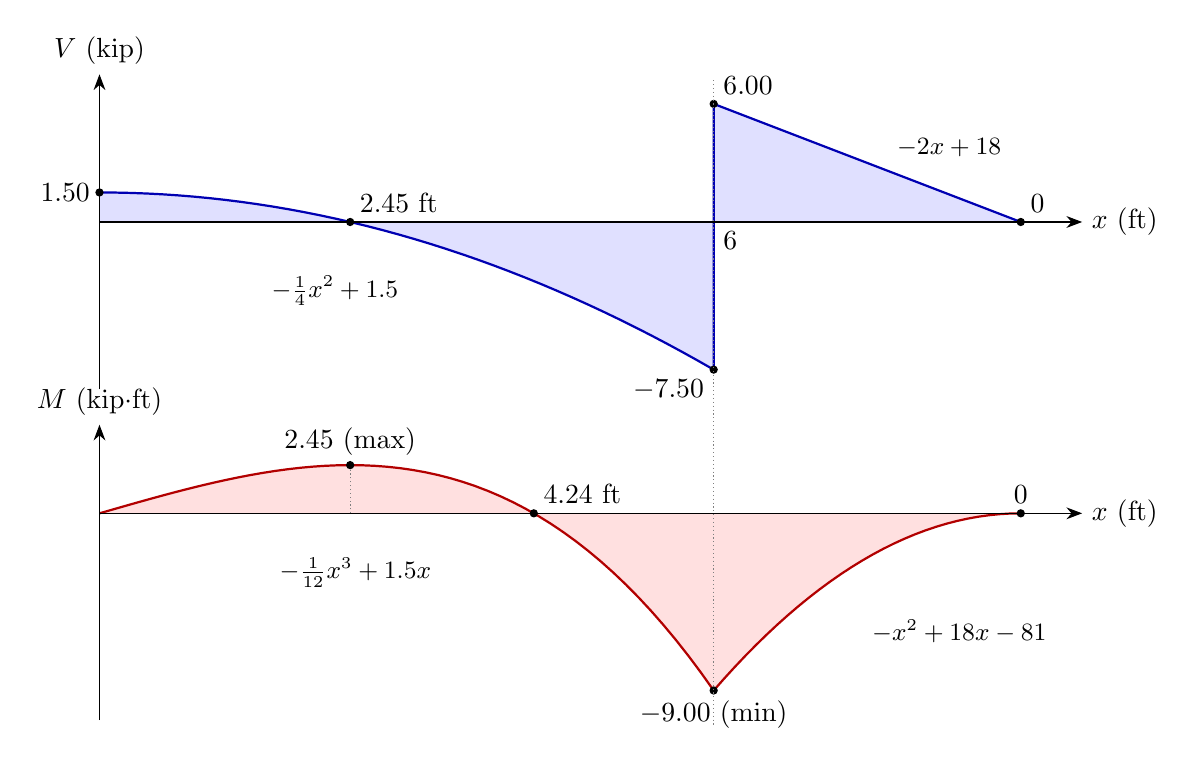
\begin{tikzpicture}[x=1cm,y=1cm]
  \begin{scope}[x=1.3cm,y=0.25cm]
    \fill[blue!12] (0,0) -- plot[domain=0:6,samples=40] (\x,{1.5-\x*\x/4}) -- (6,6) -- (9,0) -- cycle;
    \draw[thick,blue!70!black] plot[domain=0:6,samples=40] (\x,{1.5-\x*\x/4});
    \draw[thick,blue!70!black] (6,-7.5) -- (6,6) -- (9,0);
    \draw[axis] (0,0) -- (9.6,0) node[right]{$x$ (ft)};
    \draw[axis] (0,-8.5) -- (0,7.5) node[above]{$V$ (kip)};
    \fill (0,1.5) circle (1.5pt) node[left]{1.50};
    \fill (2.449,0) circle (1.5pt) node[above right]{2.45 ft};
    \fill (6,-7.5) circle (1.5pt) node[below left]{$-7.50$};
    \fill (6,6) circle (1.5pt) node[above right]{6.00};
    \fill (9,0) circle (1.5pt) node[above right]{0};
    \node[below right] at (6,0) {6};
    \node at (2.3,-3.5) {\small $-\tfrac14x^2+1.5$};
    \node at (8.3,3.8) {\small $-2x+18$};
  \end{scope}
  \begin{scope}[yshift=-3.7cm,x=1.3cm,y=0.25cm]
    \fill[red!12] (0,0) -- plot[domain=0:6,samples=50] (\x,{1.5*\x-\x*\x*\x/12}) -- plot[domain=6:9,samples=30] (\x,{-(9-\x)*(9-\x)}) -- (9,0) -- cycle;
    \draw[thick,red!70!black] plot[domain=0:6,samples=50] (\x,{1.5*\x-\x*\x*\x/12});
    \draw[thick,red!70!black] plot[domain=6:9,samples=30] (\x,{-(9-\x)*(9-\x)});
    \draw[axis] (0,0) -- (9.6,0) node[right]{$x$ (ft)};
    \draw[axis] (0,-10.5) -- (0,4.5) node[above]{$M$ (kip$\cdot$ft)};
    \draw[zero] (2.449,0) -- (2.449,2.449);
    \fill (2.449,2.449) circle (1.5pt) node[above]{2.45 (max)};
    \fill (4.243,0) circle (1.5pt) node[above right]{4.24 ft};
    \fill (6,-9) circle (1.5pt) node[below]{$-9.00$ (min)};
    \fill (9,0) circle (1.5pt) node[above]{0};
    \node at (2.5,-3) {\small $-\tfrac1{12}x^3+1.5x$};
    \node at (8.4,-6) {\small $-x^2+18x-81$};
  \end{scope}
  % alignment guides to the support
  \draw[zero] (7.8,1.8) -- (7.8,-6.4);
\end{tikzpicture}
\end{center}
\end{minipage}

\begin{finalanswer}
$0 \le x < 6$ ft: \quad $V(x) = -\tfrac14 x^2 + 1.5$ kip, \quad $M(x) = -\tfrac1{12}x^3 + 1.5x$ kip$\cdot$ft\\[4pt]
$6 < x \le 9$ ft: \quad $V(x) = -2x + 18$ kip, \quad $M(x) = -x^2 + 18x - 81$ kip$\cdot$ft\\[4pt]
$V = 0$ and $M_{\max} = 2.45$ kip$\cdot$ft at $x = 2.45$ ft; $M = 0$ at $x = 4.24$ ft; at $B$, $V$ jumps from $-7.50$ to $6.00$ kip and $M_{\min} = -9.00$ kip$\cdot$ft.
\end{finalanswer}

% =========================================================
% PROBLEM 7
% =========================================================
\clearpage
\section*{Problem 7}

\textbf{Given / Find:} Beam with a pin at $A$ ($x=0$), a roller at $B$ ($x = 12$ ft), and a 1500 lb load at the free end ($x = 16$ ft). Two identical triangular loads act: each rises from 0 to 400 lb/ft over 6 ft (from $x = 0$ to 6 and from $x = 6$ to 12). Find $V(x)$ and $M(x)$ and draw the shear and moment diagrams.

\textbf{Sketch:}

\begin{center}
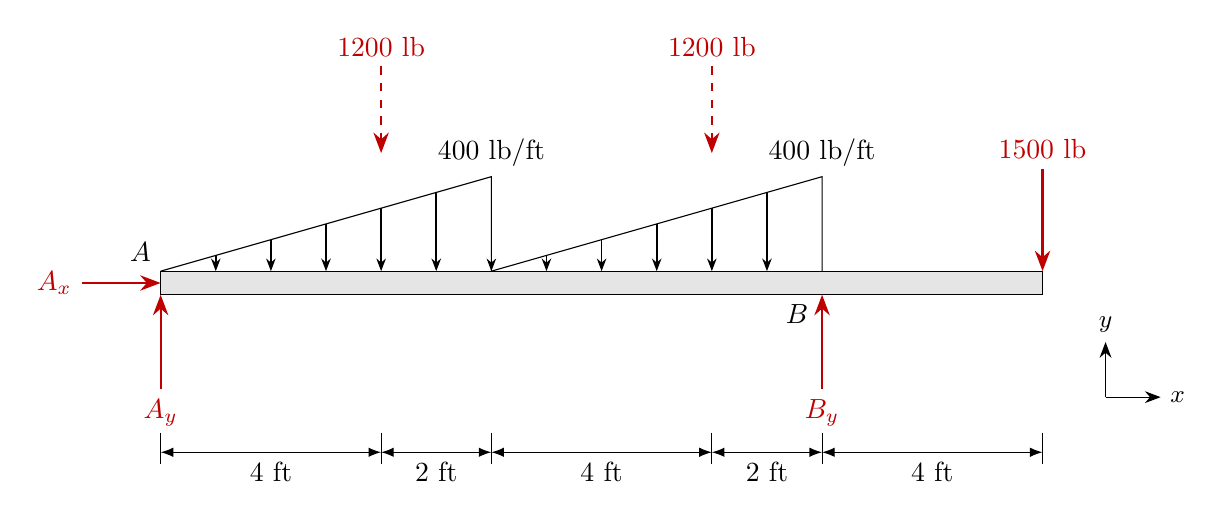
\begin{tikzpicture}[x=1cm,y=1cm]
  % 0.7 cm per ft
  \draw[beam] (0,0) rectangle (11.2,0.3);
  \node[above left] at (0,0.3) {$A$};
  \draw (0,0.3) -- (4.2,1.5) -- (4.2,0.3) -- (8.4,1.5) -- (8.4,0.3);
  \foreach \x in {0.7,1.4,...,4.2} {
    \pgfmathsetmacro{\h}{1.2*\x/4.2}
    \draw[load] (\x,0.3+\h) -- (\x,0.3);
  }
  \foreach \x in {4.9,5.6,...,8.4} {
    \pgfmathsetmacro{\h}{1.2*(\x-4.2)/4.2}
    \draw[load] (\x,0.3+\h) -- (\x,0.3);
  }
  \node[above] at (4.2,1.5) {400 lb/ft};
  \node[above] at (8.4,1.5) {400 lb/ft};
  \draw[force,dashed] (2.8,2.9) -- (2.8,1.8) node[pos=0,above]{1200 lb};
  \draw[force,dashed] (7.0,2.9) -- (7.0,1.8) node[pos=0,above]{1200 lb};
  \draw[force] (11.2,1.6) -- (11.2,0.3) node[pos=0,above]{1500 lb};
  \draw[force] (0,-1.2) -- (0,0) node[pos=0,below]{$A_y$};
  \draw[force] (-1.0,0.15) -- (0,0.15) node[pos=0,left]{$A_x$};
  \draw[force] (8.4,-1.2) -- (8.4,0) node[pos=0,below]{$B_y$};
  \node[below left] at (8.35,0) {$B$};
  \foreach \p in {0,2.8,4.2,7.0,8.4,11.2} \draw[thin] (\p,-1.75) -- (\p,-2.15);
  \draw[dimn] (0,-2) -- (2.8,-2) node[midway,below]{4 ft};
  \draw[dimn] (2.8,-2) -- (4.2,-2) node[midway,below]{2 ft};
  \draw[dimn] (4.2,-2) -- (7.0,-2) node[midway,below]{4 ft};
  \draw[dimn] (7.0,-2) -- (8.4,-2) node[midway,below]{2 ft};
  \draw[dimn] (8.4,-2) -- (11.2,-2) node[midway,below]{4 ft};
  \axesglyph{(12.0,-1.3)}
\end{tikzpicture}
\end{center}

\textbf{Solution:}

\textit{Reactions:} each triangle $\tfrac12(6)(400) = 1200\un{lb}$, at $x = 4$ and $x = 10$ ft; $A_x = 0$.
\begin{align*}
\textstyle\sum M_A &= B_y(12) - 1200(4) - 1200(10) - 1500(16) = 0\\ B_y &= \frac{4800 + 12\,000 + 24\,000}{12}\un{lb} = 3400\un{lb}\\
\textstyle\sum F_y &= A_y + 3400 - 1200 - 1200 - 1500 = 0 \;\Rightarrow\; A_y = 500\un{lb}
\end{align*}

\textit{Region 1, $0 \le x \le 6$ (left segment):} $w = 66.7x$, load $33.3x^2$ lb at $\tfrac{x}{3}$ from cut.
\begin{align*}
\textstyle\sum F_y &= 500 - 33.3x^2 - V = 0 \;\Rightarrow\; V(x) = -33.3x^2 + 500 \quad \text{(lb)}\\
\textstyle\sum M_{\text{cut}} &= M - 500x + 33.3x^2\cdot\frac{x}{3} = 0 \;\Rightarrow\; M(x) = -11.1x^3 + 500x \quad \text{(lb$\cdot$ft)}
\end{align*}

\textit{Region 2, $6 \le x < 12$ (left segment):} first triangle 1200 lb at $x = 4$; second $33.3(x-6)^2$ lb at $\tfrac{x-6}{3}$ from cut.
\begin{align*}
\textstyle\sum F_y &= 500 - 1200 - 33.3(x-6)^2 - V = 0\\
V(x) &= -700 - 33.3(x^2 - 12x + 36)\\
&= -33.3x^2 + 400x - 1900 \quad \text{(lb)}\\
\textstyle\sum M_{\text{cut}} &= M - 500x + 1200(x-4) + 33.3(x-6)^2\cdot\frac{x-6}{3} = 0\\
M(x) &= -700x + 4800\\ &\qquad - 11.1(x^3 - 18x^2 + 108x - 216)\\
&= -11.1x^3 + 200x^2 - 1900x + 7200 \quad \text{(lb$\cdot$ft)}
\end{align*}
Check: $M(6) = 600\un{lb\,ft}$ (matches region 1). The posted key's $200x$ term should be $200x^2$.

\textit{Region 3, $12 < x \le 16$ (right segment):}
\begin{align*}
\textstyle\sum F_y &= V - 1500 = 0 \;\Rightarrow\; V(x) = 1500\un{lb}\\
\textstyle\sum M_{\text{cut}} &= -M - 1500(16 - x) = 0 \;\Rightarrow\; M(x) = 1500x - 24\,000 \quad \text{(lb$\cdot$ft)}
\end{align*}

\textit{Critical values:}
\begin{align*}
V = 0:\ 500 - 33.3x^2 = 0 &\Rightarrow x = 3.87\un{ft}\\ M_{\max} &= 500(3.873) - 11.1(3.873)^3 = 1290\un{lb\,ft}\\
x = 6:\ V &= -700\un{lb},\quad M = 600\un{lb\,ft}\\
M = 0\ (u = x-6):\ u^3 + 63u - 54 = 0 &\Rightarrow u = 0.847,\quad x = 6.85\un{ft}\\
x = 12:\ V(12^-) = -1900\un{lb},\ V(12^+) &= 1500\un{lb}\ (\Delta V = B_y),\quad M(12) = -6000\un{lb\,ft}\\
x = 16:\ V &\to 0,\quad M = 0
\end{align*}

\noindent\begin{minipage}{\linewidth}
\textbf{Shear and moment diagrams:}

\begin{center}
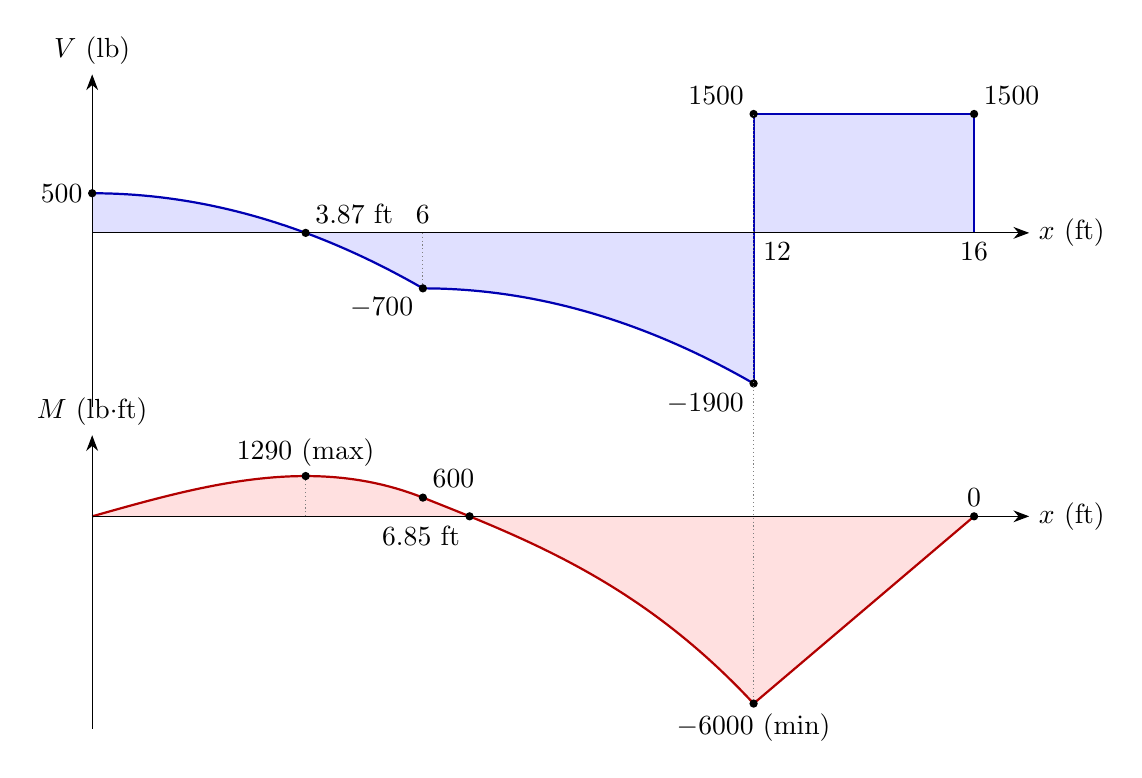
\begin{tikzpicture}[x=1cm,y=1cm]
  \begin{scope}[x=0.7cm,y=0.001cm]
    \fill[blue!12] (0,0) -- plot[domain=0:6,samples=40] (\x,{500-100*\x*\x/3}) -- plot[domain=6:12,samples=40] (\x,{-700-100*(\x-6)*(\x-6)/3}) -- (12,1500) -- (16,1500) -- (16,0) -- cycle;
    \draw[thick,blue!70!black] plot[domain=0:6,samples=40] (\x,{500-100*\x*\x/3});
    \draw[thick,blue!70!black] plot[domain=6:12,samples=40] (\x,{-700-100*(\x-6)*(\x-6)/3});
    \draw[thick,blue!70!black] (12,-1900) -- (12,1500) -- (16,1500) -- (16,0);
    \draw[axis] (0,0) -- (17,0) node[right]{$x$ (ft)};
    \draw[axis] (0,-2200) -- (0,2000) node[above]{$V$ (lb)};
    \draw[zero] (6,0) -- (6,-700);
    \fill (0,500) circle (1.5pt) node[left]{500};
    \fill (3.873,0) circle (1.5pt) node[above right]{3.87 ft};
    \fill (6,-700) circle (1.5pt) node[below left]{$-700$};
    \fill (12,-1900) circle (1.5pt) node[below left]{$-1900$};
    \fill (12,1500) circle (1.5pt) node[above left]{1500};
    \fill (16,1500) circle (1.5pt) node[above right]{1500};
    \node[above] at (6,0) {6};
    \node[below right] at (12,0) {12};
    \node[below] at (16,0) {16};
  \end{scope}
  \begin{scope}[yshift=-3.6cm,x=0.7cm,y=0.0004cm]
    \fill[red!12] (0,0) -- plot[domain=0:6,samples=50] (\x,{500*\x-11.1111*\x*\x*\x}) -- plot[domain=6:12,samples=50] (\x,{600-700*(\x-6)-11.1111*(\x-6)*(\x-6)*(\x-6)}) -- (16,0) -- cycle;
    \draw[thick,red!70!black] plot[domain=0:6,samples=50] (\x,{500*\x-11.1111*\x*\x*\x});
    \draw[thick,red!70!black] plot[domain=6:12,samples=50] (\x,{600-700*(\x-6)-11.1111*(\x-6)*(\x-6)*(\x-6)});
    \draw[thick,red!70!black] (12,-6000) -- (16,0);
    \draw[axis] (0,0) -- (17,0) node[right]{$x$ (ft)};
    \draw[axis] (0,-6800) -- (0,2600) node[above]{$M$ (lb$\cdot$ft)};
    \draw[zero] (3.873,0) -- (3.873,1291);
    \fill (3.873,1291) circle (1.5pt) node[above]{1290 (max)};
    \fill (6,600) circle (1.5pt) node[above right]{600};
    \fill (6.847,0) circle (1.5pt) node[below left]{6.85 ft};
    \fill (12,-6000) circle (1.5pt) node[below]{$-6000$ (min)};
    \fill (16,0) circle (1.5pt) node[above]{0};
  \end{scope}
  \draw[zero] (8.4,1.5) -- (8.4,-5.9);
\end{tikzpicture}
\end{center}
\end{minipage}

\begin{finalanswer}
$0 \le x \le 6$ ft: \quad $V(x) = -33.3x^2 + 500$ lb, \quad $M(x) = -11.1x^3 + 500x$ lb$\cdot$ft\\[4pt]
$6 \le x < 12$ ft: \quad $V(x) = -33.3x^2 + 400x - 1900$ lb, \quad $M(x) = -11.1x^3 + 200x^2 - 1900x + 7200$ lb$\cdot$ft\\[4pt]
$12 < x \le 16$ ft: \quad $V(x) = 1500$ lb, \quad $M(x) = 1500x - 24\,000$ lb$\cdot$ft\\[4pt]
$M_{\max} = 1290$ lb$\cdot$ft at $x = 3.87$ ft ($V = 0$); $M = 0$ at $x = 6.85$ ft; $M_{\min} = -6000$ lb$\cdot$ft at $B$, where $V$ jumps from $-1900$ to $1500$ lb.
\end{finalanswer}

% =========================================================
% PROBLEM 8
% =========================================================
\clearpage
\section*{Problem 8}

\textbf{Given / Find:} Cable $ABCDE$ hangs between supports $A$ and $E$ at the same elevation. Horizontal spacing: $A$--$B$ 4 m, $B$--$C$ 6 m, $C$--$D$ 3 m, $D$--$E$ 2 m. Loads: 4 kN at $B$, $P$ at $C$, 6 kN at $D$. $D$ hangs 3 m below $E$, and segment $BC$ must stay horizontal. Find $P$, the sag $y_B$, and the maximum cable tension.

\textbf{Sketch:}

\begin{center}
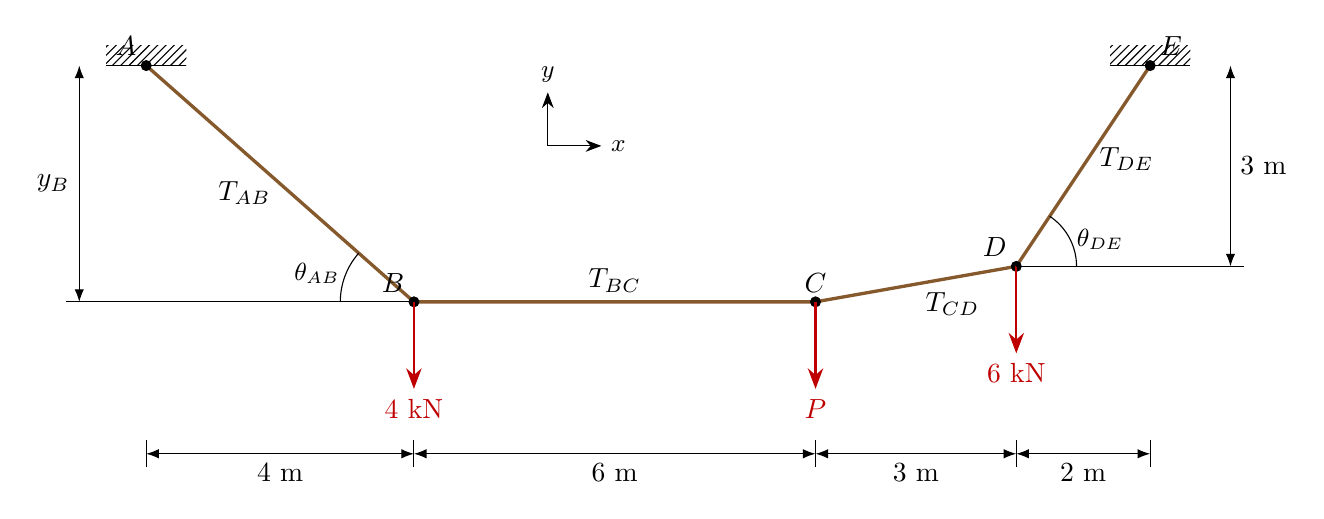
\begin{tikzpicture}[x=0.85cm,y=0.85cm]
  \coordinate (A) at (0,0);
  \coordinate (B) at (4,-3.53);
  \coordinate (C) at (10,-3.53);
  \coordinate (D) at (13,-3);
  \coordinate (E) at (15,0);
  \fill[pattern=north east lines] (-0.6,0) rectangle (0.6,0.3);
  \fill[pattern=north east lines] (14.4,0) rectangle (15.6,0.3);
  \draw (-0.6,0) -- (0.6,0); \draw (14.4,0) -- (15.6,0);
  \draw[very thick,brown!70!black] (A) -- (B) -- (C) -- (D) -- (E);
  \foreach \p in {A,B,C,D,E} \fill (\p) circle (2pt);
  \node[above left] at (A) {$A$};
  \node[above left] at (B) {$B$};
  \node[above] at (C) {$C$};
  \node[above left] at (D) {$D$};
  \node[above right] at (E) {$E$};
  \draw[force] (B) -- ++(0,-1.3) node[below]{4 kN};
  \draw[force] (C) -- ++(0,-1.3) node[below]{$P$};
  \draw[force] (D) -- ++(0,-1.3) node[below]{6 kN};
  % tension labels
  \node[left] at (2,-1.9) {$T_{AB}$};
  \node[above] at (7,-3.53) {$T_{BC}$};
  \node[below right] at (11.5,-3.25) {$T_{CD}$};
  \node[right] at (14.1,-1.4) {$T_{DE}$};
  % angles
  \draw[thin] (B) -- (2.6,-3.53);
  \draw (4,-3.53) ++(-1.1,0) arc (180:138.6:1.1);
  \node at (2.55,-3.1) {\small $\theta_{AB}$};
  \draw (13,-3) ++(0.9,0) arc (0:56.3:0.9);
  \node at (14.25,-2.6) {\small $\theta_{DE}$};
  % dims
  \draw[dimn] (-1.0,0) -- (-1.0,-3.53) node[midway,left]{$y_B$};
  \draw[thin] (-1.2,-3.53) -- (B);
  \draw[dimn] (16.2,0) -- (16.2,-3) node[midway,right]{3 m};
  \draw[thin] (D) -- (16.4,-3);
  \foreach \p in {0,4,10,13,15} \draw[thin] (\p,-5.6) -- (\p,-6.0);
  \draw[dimn] (0,-5.8) -- (4,-5.8) node[midway,below]{4 m};
  \draw[dimn] (4,-5.8) -- (10,-5.8) node[midway,below]{6 m};
  \draw[dimn] (10,-5.8) -- (13,-5.8) node[midway,below]{3 m};
  \draw[dimn] (13,-5.8) -- (15,-5.8) node[midway,below]{2 m};
  \draw[axis] (6,-1.2) -- ++(0.8,0) node[right]{\small $x$};
  \draw[axis] (6,-1.2) -- ++(0,0.8) node[above]{\small $y$};
\end{tikzpicture}

\vspace{0.3cm}
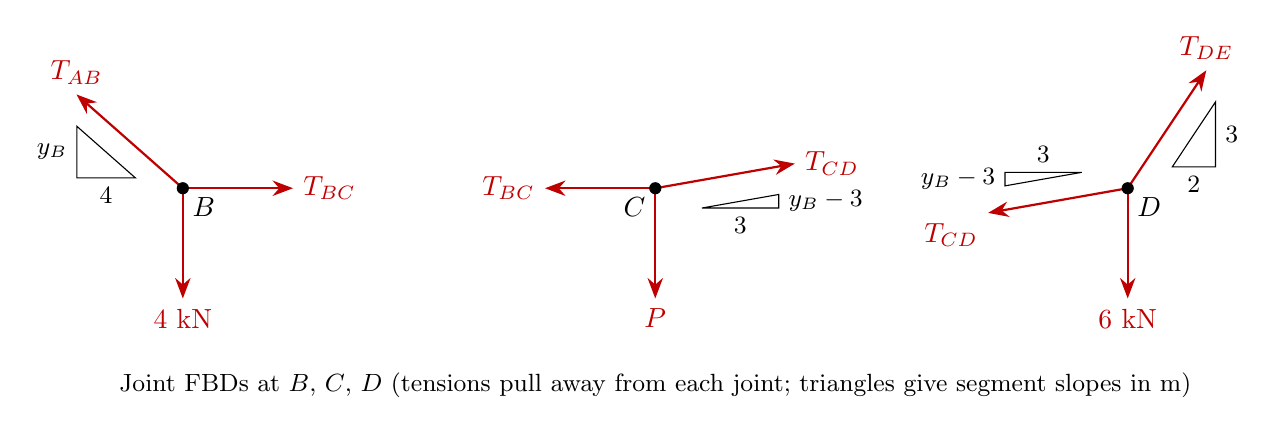
\begin{tikzpicture}[x=1cm,y=1cm]
  % ---- joint B ----
  \draw[force] (0,0) -- (-1.350,1.191) node[above]{$T_{AB}$};
  \draw[force] (0,0) -- (1.4,0) node[right]{$T_{BC}$};
  \draw[force] (0,0) -- (0,-1.4) node[below]{4 kN};
  \fill (0,0) circle (2.2pt);
  \node[below right] at (0,0) {$B$};
  \draw[thin] (-0.603,0.132) -- (-1.346,0.132) -- (-1.346,0.787) -- cycle;
  \node[below] at (-0.975,0.132) {\small 4};
  \node[left] at (-1.346,0.460) {\small $y_B$};
  % ---- joint C ----
  \begin{scope}[xshift=6.0cm]
  \draw[force] (0,0) -- (-1.4,0) node[left]{$T_{BC}$};
  \draw[force] (0,0) -- (1.773,0.313) node[right]{$T_{CD}$};
  \draw[force] (0,0) -- (0,-1.4) node[below]{$P$};
  \fill (0,0) circle (2.2pt);
  \node[below left] at (0,0) {$C$};
  \draw[thin] (0.593,-0.251) -- (1.568,-0.251) -- (1.568,-0.079) -- cycle;
  \node[below] at (1.080,-0.251) {\small 3};
  \node[right] at (1.568,-0.165) {\small $y_B-3$};
  \end{scope}
  % ---- joint D ----
  \begin{scope}[xshift=12.0cm]
  \draw[force] (0,0) -- (-1.773,-0.313) node[below left]{$T_{CD}$};
  \draw[force] (0,0) -- (0.998,1.498) node[above]{$T_{DE}$};
  \draw[force] (0,0) -- (0,-1.4) node[below]{6 kN};
  \fill (0,0) circle (2.2pt);
  \node[below right] at (0,0) {$D$};
  \draw[thin] (-0.584,0.202) -- (-1.559,0.202) -- (-1.559,0.030) -- cycle;
  \node[above] at (-1.071,0.202) {\small 3};
  \node[left] at (-1.559,0.116) {\small $y_B-3$};
  \draw[thin] (0.566,0.272) -- (1.115,0.272) -- (1.115,1.096) -- cycle;
  \node[below] at (0.840,0.272) {\small 2};
  \node[right] at (1.115,0.684) {\small 3};
  \end{scope}
  \node at (6.0,-2.5) {\small Joint FBDs at $B$, $C$, $D$ (tensions pull away from each joint; triangles give segment slopes in m)};
\end{tikzpicture}
\end{center}

\textbf{Solution:}

\textit{Geometry} ($A$, $E$ level; $B$, $C$ at depth $y_B$; $D$ at 3 m):
\[
\tan\theta_{AB} = \frac{y_B}{4}, \qquad \theta_{BC} = 0, \qquad \tan\theta_{CD} = \frac{y_B - 3}{3}, \qquad \tan\theta_{DE} = \frac{3}{2}
\]

$\sum F_x = 0$ at each joint $\Rightarrow$ constant horizontal component $T_H = T_{BC}$; vertical component of each segment $= T_H\tan\theta$.

\textit{$\sum F_y = 0$ at each joint:}
\begin{align}
\text{Joint } B:\quad T_H\frac{y_B}{4} - 4\un{kN} &= 0 \tag{1}\\
\text{Joint } C:\quad T_H\frac{y_B - 3}{3} - P &= 0 \tag{2}\\
\text{Joint } D:\quad T_H\frac{3}{2} - T_H\frac{y_B - 3}{3} - 6\un{kN} &= 0 \tag{3}
\end{align}

\textit{Solve (1) and (3) for $T_H$, $y_B$:} from (1), $T_H = 16/y_B$; into (3):
\begin{align*}
\frac{16}{y_B}\left[\frac32 - \frac{y_B - 3}{3}\right] = 6
\;\Rightarrow\; \frac{16}{y_B}\cdot\frac{15 - 2y_B}{6} = 6
\;\Rightarrow\; 240 - 32y_B = 36y_B
\;\Rightarrow\; y_B = \frac{240}{68} = 3.529\un{m}
\end{align*}
\[
T_H = \frac{16\un{kN\,m}}{3.529\un{m}} = 4.533\un{kN}
\]
From (2):
\[
P = (4.533\un{kN})\frac{3.529 - 3}{3} = (4.533\un{kN})(0.1765) = 0.800\un{kN}
\]

\textit{Tensions,} $T = T_H\sqrt{1 + \tan^2\theta}$:
\begin{align*}
T_{AB} &= 4.533\sqrt{1 + (3.529/4)^2} = 4.533(1.334) = 6.05\un{kN}\\
T_{BC} &= T_H = 4.53\un{kN}\\
T_{CD} &= 4.533\sqrt{1 + (0.529/3)^2} = 4.533(1.015) = 4.60\un{kN}\\
T_{DE} &= 4.533\sqrt{1 + (3/2)^2} = 4.533(1.803) = 8.17\un{kN}
\end{align*}

\textit{Check:} $T_H(y_B/4 + 3/2) = 10.8\un{kN} = 4 + 0.8 + 6$ \checkmark

\begin{finalanswer}
$P = 0.800\un{kN}$, \quad $y_B = 3.53\un{m}$, \quad $T_{\max} = T_{DE} = 8.17\un{kN}$
\end{finalanswer}

\end{document}